\subsection{Style Tab}
\label{sec:geoview_style}

\begin{figure}[H]
   \centering
    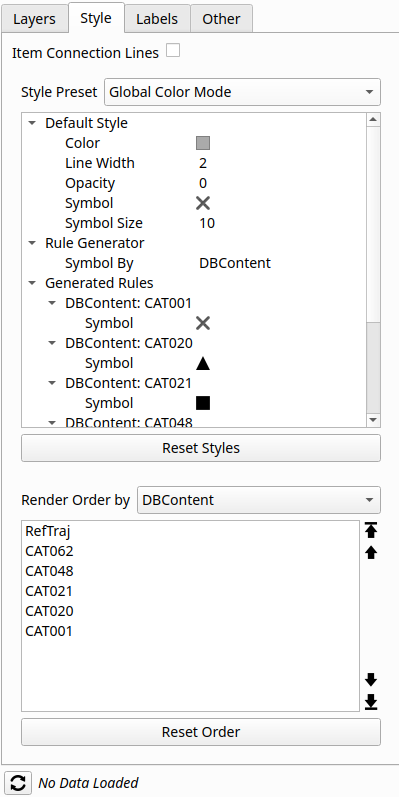
\includegraphics[width=8cm,frame]{figures/geoview_style_tab.png}
  \caption{Geographic View Style tab}
\end{figure}

The 'Style' tab contains:

\begin{itemize}
 \item Item Connection Lines: Connection-lines checkbox (see \nameref{sec:item_connection_lines})
 \item Style Preset: Preset selection and per-preset configuration (see \nameref{sec:style})
 \item Render Order: Drawing order of DBContents (see \nameref{sec:render_order})
\end{itemize}
\ \\

\subsubsection{Item Connection Lines}
\label{sec:item_connection_lines}

If the 'Item Connection Lines' checkbox is set, connection lines between all target reports in the last layer are drawn, except for the 'None' layer. \\

Please note that connection lines for target reports with a time-of-day difference larger than 5 minutes will be omitted. \\

\begin{figure}[H]
    \centering
    \hspace*{-2.5cm}
    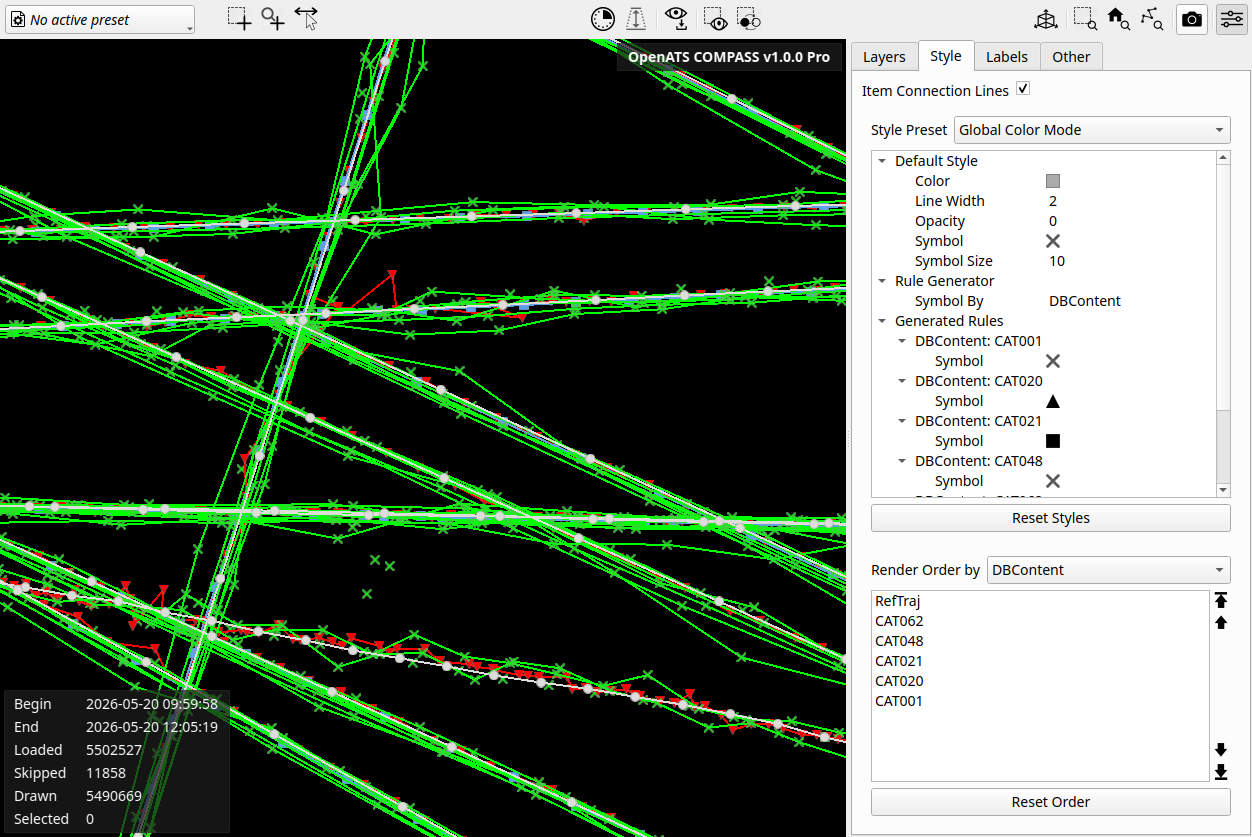
\includegraphics[width=19cm,frame]{figures/geoview_connect_lines.png}
  \caption{Geographic View Data with lines}
\end{figure}

Please \textbf{note} that changing this value requires a redraw.

\subsubsection{Style Preset}
\label{sec:style}

This section contains the 'Style Preset' combo box, the preset configuration area, and a 'Reset Styles' button that clears all style presets to their default values. \\

The following presets exist (default 'Color by Speed'):

\begin{itemize}
 \item Global Color Mode: Uses the global color mode setting from the main application
 \item Color by Item: Colors target reports by the item color assigned in the Item Mode panel (see \nameref{sec:geo_item_mode}). One color per grouped item (e.g. per UTN, per Aircraft Address, per Mode 3/A Code), depending on the current Item Mode grouping. Replaces the previous 'Layer Color per ...' presets.
 \item Color by ADSB MOPS: V0 / V1 / V2 colors for CAT021 ADS-B target reports
 \item Color by ADSB Position Quality: NUCp / NACp colors for CAT021 ADS-B target reports
 \item Color by Detection Type: Radar detection type (PSR, SSR, PSR+SSR, Mode S, ...)
 \item Color by Flight Level: Gradient by Mode C flight level, per DBContent
 \item Color by Line ID: Color per line ID (L1-L4), with the symbol still driven by DBContent
 \item Color by Num Contributing Sensors: Number of contributing sensors of a CAT062 target report (sum of REF.CSN.REP and REF.CST.REP)
 \item Color by Speed: Gradient by ground speed
 \item Color by Track Age: Color by track age, with 4 intervals plus 'None'
 \item Color by Track Angle: Color by direction of movement (N / E / S / W gradient)
\end{itemize}
\ \\

Per-preset parameters (e.g. colors per interval, time interval used, variable used) can be adapted in the configuration tree below the combo box. Changes are applied immediately to the data. \\

Please note that after changing the active preset a redraw or reload may be triggered automatically. \\


\includegraphics[width=0.5cm]{../../data/icons/hint.png} Please also note that for presets relying on a specific data variable (e.g. flight level, ADS-B quality, contributing sensors), the corresponding data has to be present in the loaded target reports; otherwise the affected target reports are styled with the 'None' color.

\subsubsection{Style Example}

As an example, the 'Color by Flight Level' preset applied to a mixed dataset:

\begin{figure}[H]
    \centering
    \hspace*{-2.5cm}
    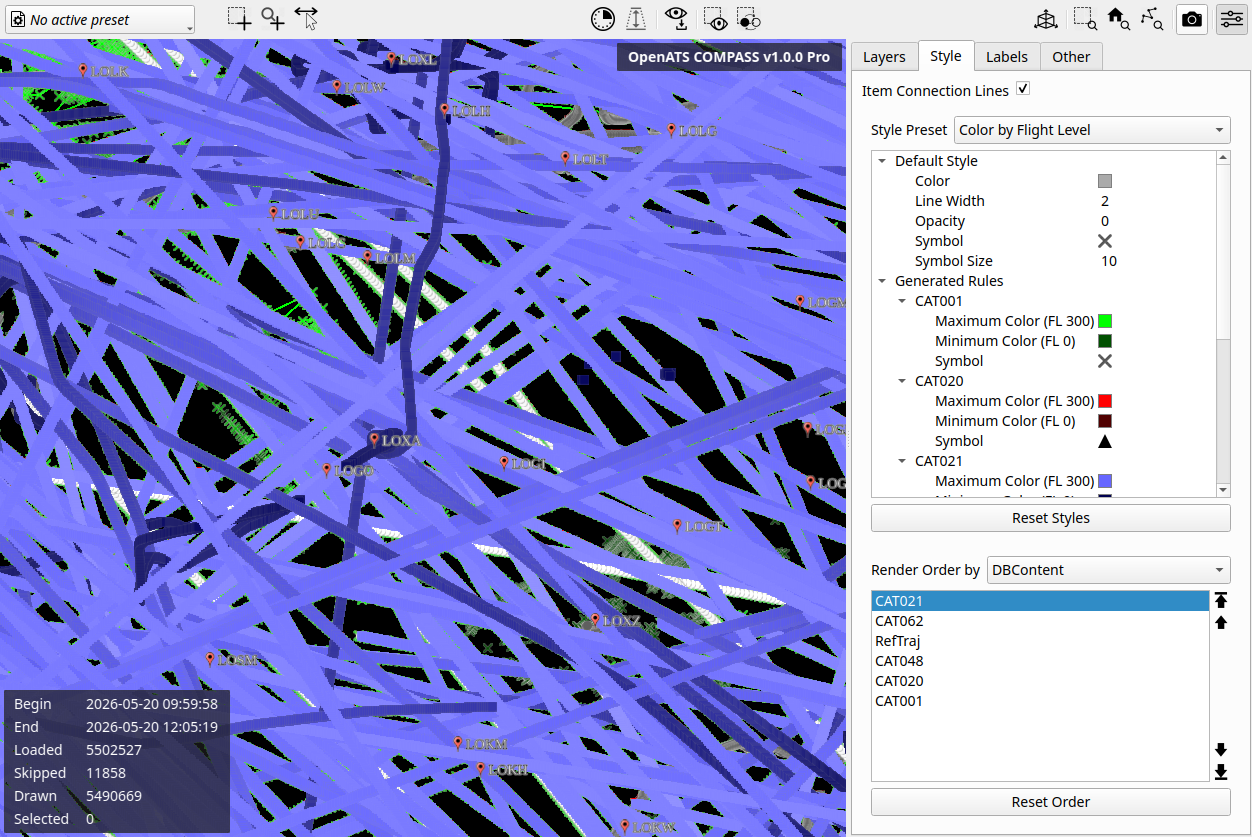
\includegraphics[width=19cm,frame]{figures/geoview_style_flight_level.png}
  \caption{Geographic View Color by Flight Level}
\end{figure}

\subsubsection{Render Order}
\label{sec:render_order}

In the render order widget, the drawing order of the drawn data is specified. The one at the top is drawn last (over all others), so it is useful to move the most important DBContent (for the current inspection) to the top.

\begin{figure}[H]
    \centering
    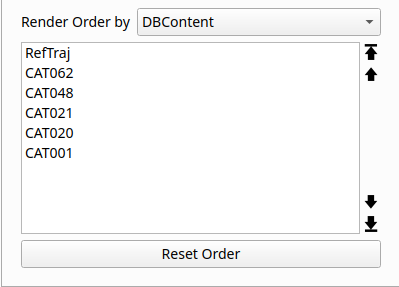
\includegraphics[width=8cm,frame]{figures/geoview_render_order.png}
  \caption{Geographic View render order}
\end{figure}

Using the 'Render Order by' combo, the drawing order can be defined based on:

\begin{itemize}
 \item DBContent: Data source type (e.g. Tracker, Radar, ...)
 \item DS ID: Data source (e.g. Tracker1, Tracker2, Radar3, ...)
 \item DS ID+Line ID: Data source and Line ID (e.g. Tracker1 L1, Tracker1 L2, ...)
\end{itemize}
\ \\

To change the drawing order click on the item to move and use the buttons on the right side. Please note that no redraw is required and that the drawing order is persisted in the configuration. \\

\begin{itemize}
 \item \includegraphics[width=0.5cm]{../../data/icons/top.png} Move to Top: Move item to top position
 \item \includegraphics[width=0.5cm]{../../data/icons/up.png} Move Up: Move item one position up
 \item \includegraphics[width=0.5cm]{../../data/icons/down.png} Move Down: Move item one position down
 \item \includegraphics[width=0.5cm]{../../data/icons/bottom.png} Move to Bottom: Move item to the bottom position
\end{itemize}
\ \\

The 'Reset Order' button below the list resets the current render order to its default.
